% +--------------------------------------------------------------------+
% | LaTeX Template                                                     |
% | for K-State Electronic Theses, Dissertations, and Reports          |
% |                                                                    |
% | Comments and guidelines for using the template are shown           |
% | within boxes like this one.                                        |
% |                                                                    |
% | Revised 6/30/06                                                    |
% | 9/14/06: Removed typos                                             |
% +--------------------------------------------------------------------+

% +--------------------------------------------------------------------+
% | Your paper should contain the following sections, except where     |
% | indicated as optional, in the order shown.  Also, all headings     |
% | shown with an asterisk (*) must be centered and in uppercase       |
% | letters:                                                           |
% |                                                                    |
% | Abstract Title Page (doctoral dissertations only)                  |
% | ABSTRACT* (doctoral dissertations only)                            |
% | Title Page                                                         |
% | Copyright Page (Optional - only needed if copyrighting)            |
% | ABSTRACT *                                                         |
% | TABLE OF CONTENTS *                                                |
% | LIST OF FIGURES *                                                  |
% | LIST OF TABLES*                                                    |
% | ACKNOWLEDGMENTS* (Optional)                                        |
% | DEDICATION * (Optional)                                            |
% | PREFACE * (Optional)                                               |
% | Individual Chapters                                                |
% | References and/or bibliography                                     |
% | Appendices (as needed)                                             |
% +--------------------------------------------------------------------+

% +--------------------------------------------------------------------+
% | The LaTex keyword \documentclass selects a particular class to     |
% | associate with the document.  The current documentclass            |
% | {class_diss} generates a Table of Contents that has leading dots   |
% | only on chapter subheadings.  If you prefer a Table of Contents    |
% | that has leading dots for all entries, replace {class_diss}        |
% | with {Mydiss} in the command below.                                |
% |                                                                    |
% +--------------------------------------------------------------------+

\documentclass[final,12pt,oneside]{class_diss}

% +--------------------------------------------------------------------+
% | The following command sets the bibliography style to American
% | Institute of Physics (AIP).  Other styles are available in the
% | styles directory.  To use a different style, replace "aip" with
% | the filename of the style you want to use.
% +--------------------------------------------------------------------+

\bibliographystyle{styles/plain}

\usepackage[utf8]{inputenc}
\usepackage[T1]{fontenc}
\usepackage[USenglish,spanish]{babel}

%\usepackage{     caption2} % Customize captions a bit more
\usepackage{      amsmath} % American Mathematics Society standards
%\usepackage{      wrapfig} % Wraps text around a figure or table
\usepackage{     graphicx} % Extended graphics package.
%\usepackage{     fancyhdr} % Efficiently handles headers and footers
%\usepackage{       braket} % Bra-Ket notation package
%\usepackage{     mathrsfs} % Specialized Math fonts (Hamiltonian, etc.)
%\usepackage{boxedminipage} % Boxed text can be produced
%\usepackage{     setspace} % Controls line spacing via \begin{space}

\usepackage{amsxtra}
\usepackage{amssymb}
\usepackage{amsthm}
\usepackage{latexsym}

% +--------------------------------------------------------------------+
% | The color package allows one to select colors for hyperlinking     |
% | (see below).                                                       |
% +--------------------------------------------------------------------+

\usepackage[usenames]{color}

% +--------------------------------------------------------------------+
% | Colors defined for use with this template.                         |
% +--------------------------------------------------------------------+

\definecolor{  Pink}{rgb}{1.0, 0.5, 0.5}
\definecolor{Maroon}{rgb}{0.8, 0.0, 0.0}

% +--------------------------------------------------------------------+
% | In the commands below, we use the 'natbib' package, and specify    |
% | the 'sort&compress' option, which condenses                        |
% | citations from (1,2,3,5,9,10,11) to (1-3,5,9-11).  The 'bibpunct'  |
% | option selects various parameters for how the citation will be     |
% | displayed.  In this case, only the comma (separation between       |
% | citations) and the 's' (superscript) arguments are chosen.  The    |
% | other curly braces deal with how to 'wrap' the citation (using     |
% | parentheses, brackets, etc.) and are not needed for the chosen     |
% | style.                                                             |
% +--------------------------------------------------------------------+

\usepackage[sort&compress]{natbib}
\bibpunct{}{}{,}{s}{}{}
\usepackage{hypernat}

% +--------------------------------------------------------------------+
% | Lastly, the hyperref package allows one to hyperlink cross-        |
% | references and figures in a LaTeX document.                        |
% +--------------------------------------------------------------------+

\usepackage[pdftex, plainpages=false, pdfpagelabels]{hyperref}

\hypersetup{
   linktocpage=true,
   colorlinks=true,
   bookmarks=true,
   citecolor=blue,
   urlcolor=red,
   linkcolor=Maroon,
   citebordercolor={1 0 0},
   urlbordercolor={1 0 0},
   linkbordercolor={.7 .8 .8},
   breaklinks=true,
   pdfpagelabels=true,
}

\topmargin      = -0.56in
\textheight     =  8.60in
\textwidth      =  6.46in
\oddsidemargin  =  0.02in

\begin{document}
   \setcounter{page}{-1}

   \newpage
\thispagestyle{empty}
\begin{center}
   \vspace{1cm}
   {\Large A FAST IMPLEMENTATION OF PARALLEL SNAPSHOT ISOLATION}\\
   \vspace{1cm}
   {\large Borja Arnau de Régil Basáñez}\\
   \vspace{0.85cm}
   
\includegraphics[height=2.5in]{figures/escudo.png}

   \vspace{0.85cm}
   Trabajo de Fin de Grado del Grado en Ingeniería\\
   Informática\\

   \vspace{0.2cm}
   Facultad de Informática,\\
   Universidad Complutense de Madrid \\

   \vspace{1cm}
   Junio 2020
\end{center}

{\raggedleft
   \vspace{2cm}
   Director: Maria Victoria López López\\
   Co-directores: Alexey Gotsman \& Manuel Bravo\\
}

   \pdfbookmark[0]{Portada}{PDFPortadaPage}

   \newpage
\thispagestyle{empty}
\begin{center}
   {\bf \Huge Autorización de difusión}
   \vspace{1cm}

   \large Borja Arnau de Régil Basáñez\\
   \vspace{0.5cm}
   \today\\
   \vspace{0.5cm}
\end{center}

El abajo firmante, matriculado en el Grado de Ingeniería Informática de la Facultad de Informática, autoriza a la Universidad Complutense de Madrid (UCM) a difundir y utilizar con fines académicos, no comerciales y mencionando expresamente a su autor el presente Trabajo Fin de Grado: ``A fast implementation of Parallel Snapshot Isolation'', realizado durante el curso académico 2019-2020 bajo la dirección de Maria Victoria López López en el Departamento de Arquitectura de Computadores y Automática, y con la colaboración externa de dirección de Alexey Gotsman; y a la Biblioteca de la UCM a depositarlo en el Archivo Institucional E-Prints Complutense con el objeto de incrementar la difusión, uso e impacto del trabajo en Internet y garantizar su preservación y acceso a largo plazo.


   \pdfbookmark[0]{Autorización}{PDFAutorizacionPage}

% +--------------------------------------------------------------------+
% | On the line below, set the number to represent the page number of
% | the Table of Contents page.  For example, if the Table of Contents
% | page is the 8th page of your document, enter 8 in the brackets.  This
% | number may vary, depending on the length of your abstract.
% |
% | Numbers do not appear on the title and abstract pages, but they are
% | included in the page count.  The Table of Contents page is the
% | first page on which page numbers are displayed.
% +--------------------------------------------------------------------+

   \pagenumbering{roman}
   \setcounter{page}{-1}
   \phantomsection
   \selectlanguage{USenglish}
   \tableofcontents
   %\listoffigures
   %\listoftables

   \newpage

\begin{center}
{\bf \Huge Acknowledgements}
\end{center}

\vspace{1cm}

To my advisors Maria Victoria López López at Universidad Complutense de Madrid, and Alexey Gotsman and Manuel Bravo at the IMDEA Software Institute, for their guidance and support, and for giving me the opportunity to work along them.\\

I also thank Christopher Meiklejohn, who allowed me to work with him, and gave me the opportunity to discover the IMDEA Software Institute. To my colleagues at IMDEA, for giving advice and offering a helping hand.\\

Finally, to my girlfriend Paula, and my family, for their love, patience and support.\\

   \phantomsection
   \addcontentsline{toc}{chapter}{Acknowledgements}

   \newpage
\begin{center}
    {\bf \Huge Dedication}
\end{center}
\vspace{1cm}
\setlength{\baselineskip}{0.8cm}

Texto...
   \phantomsection
   \addcontentsline{toc}{chapter}{Dedication}

   \newpage

\begin{center}
{\bf \Huge Abstract}
\end{center}

\vspace{1cm}

\todo{Keep this paragraph, merge the next two into a single one, to say that both PSI and NMSI help. However, sometimes the programmer wants stronger consistency (SI). In this work, we propose a variant of PSI that allows stronger consistency, while still being ``fast''.}

Most distributed database systems use weak consistency protocols to avoid the
performance penalty of coordinating replicas. However, these protocols impose
on the programmers the need to reason about possible anomalies, and the need
to implement conflict resolution mechanisms in application code.

Parallel Snapshot Isolation (PSI) has been proposed as a solution to this
problem, however, it suffers a significant abort rate due to stale reads,
given that transactions are forced to read from a fixed snapshot of versions
once they start.

In contrast, the recently proposed Non-Monotonic Snapshot Isolation (NMSI)
protocol allows transactions to read versions of data committed after it
started, leading to a lower abort rate and increased scalability. In spite
of this, the proposed implementation uses a complex clock mechanism to ensure
consistent snapshots.

In this work, we'll show a implementation of the NMSI protocol using logical
clocks to ensure consistent snapshots and simple conflict resolution, and
compare it against the previous implementation. In addition, we perform a
comparative study of different consistency protocol implementations, showing
that NMSI can offer similar performance to weaker protocols while providing
stronger guarantees.

\vspace{1cm}

\begin{center}
{\bf \Large Keywords}
\end{center}

\vspace{0.5cm}

Consistency models, Transactions, Parallel Snapshot Isolation, Non-Monotonic Snapshot Isolation, Concurrency control.

   \phantomsection
   \addcontentsline{toc}{chapter}{Abstract}

   \newpage

\begin{center}
{\bf \Huge Resumen}
\end{center}

\vspace{1cm}

La mayoría de las bases de datos distribuidas usan protocolos de consistencia débil
para evitar la penalización de rendimiento que supone la coordinación de las distintas
réplicas. Sin embargo, dichos protocolos imponen en los programadores la necesidad de
razonar sobre posibles anomalías, así como implementar mecanismos de resolución de
conflictos en el código de las aplicaciones.

El protocolo PSI (Parallel Snapshot Isolation) se ha propuesto como una posible solución,
sin embargo sufre de una significativa tasa de abortos debido a lecturas de datos antiguos,
dado que las transaciones están obligadas a leer de una instantánea fijada en el momento
en que comienzan.

En contraste, el protocolo NMSI (Non-Monotonic Snapshot Isolation) propuesto recientemente
permite a las transacciones leer versiones de datos confirmados después de su comienzo,
lo que conlleva una tasa de cancelación más baja y una mayor escalabilidad. A pesar de esto,
la implementación propuesta utiliza un mecanismo de relojes complejo para garantizar instantáneas
consistentes.

En este trabajo, mostraremos una implementación del protocolo NMSI usando relojes lógicos
para garantizar instantáneas consistentes y una resolución de conflictos simple, comparándola
con la implementación anterior. Además, realizamos un estudio comparativo de diferentes
implementaciones de protocolos de consistencia, mostrando que NMSI puede ofrecer un rendimiento
similar a los protocolos más débiles mientras proporciona garantías mas fuertes.

\vspace{1cm}

\begin{center}
{\bf \Large Palabras clave}
\end{center}

\vspace{0.5cm}

Modelos de Consistencia, Transacciones, Control de Concurrencia.

   \phantomsection
   \addcontentsline{toc}{chapter}{Resumen}

% +--------------------------------------------------------------------+
% | We use arabic (1, 2, 3...) page numbering starting from page 1.    |
% | Note, however, that there are many pages where this is not the     |
% | desired behavior - such as the Title page, or abstract.  In these  |
% | cases, we can use \thispagestyle{empty} to suppress page numbers,  |
% | and other general style issues that we've defined globally.        |
% +--------------------------------------------------------------------+

   \newpage
   \pagenumbering{arabic}
   \setcounter{page}{1}

   % +--------------------------------------------------------------------+
% | Sample Chapter
% |
% | This file provides examples of how to
% | - insert a figure with a caption
% | - construct a table with a caption
% | - create subsections within the chapter
% | - insert a reference to a Figure or Table
% | - make a citation
% +--------------------------------------------------------------------+

\cleardoublepage

% +--------------------------------------------------------------------+
% | Replace "Chapter Title" below with the title of your chapter.  LaTeX
% | will automatically number the chapters.
% +--------------------------------------------------------------------+

\chapter{Chapter Title}
%\label{ch:chapter1}
\label{makereference}

In this chapter, there will be examples of various features you
may want to incorporate into your document. Here's an example of a
figure inserted into the text:

\begin{figure}[htb]%t=top, b=bottom, h=here

    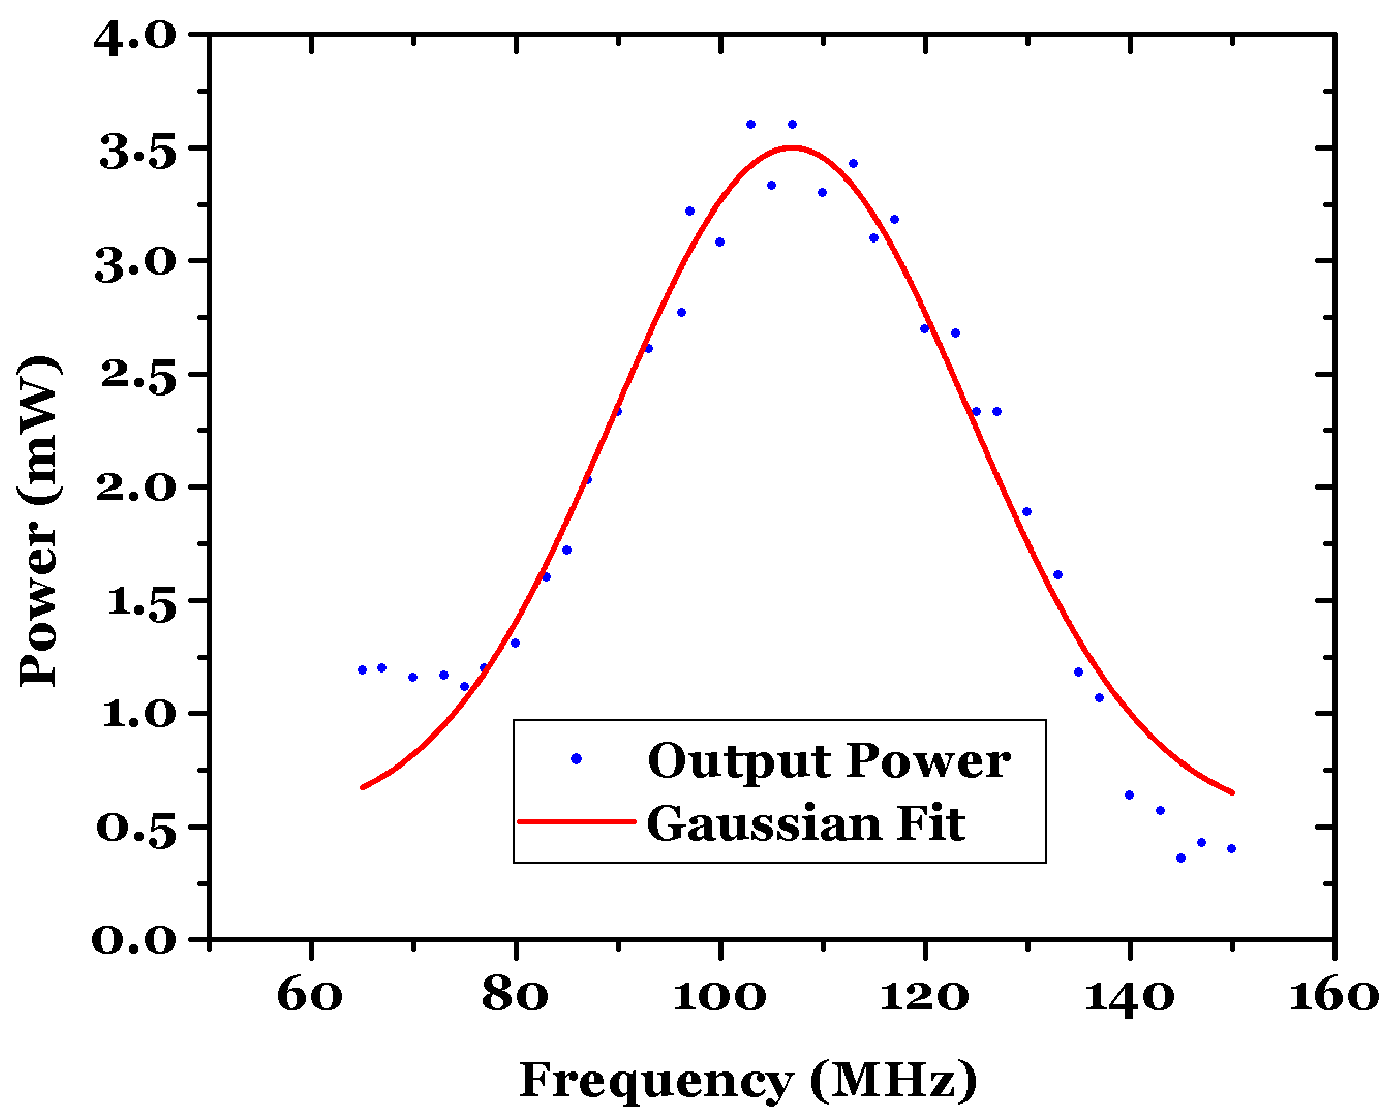
\includegraphics[height=2.5in]{figures/graph.png}

    \caption[Optional: Short caption to appear in List of
    Figures]{Full caption to appear below the Figure}

    \label{figure1}
\end{figure}

% +--------------------------------------------------------------------+
% |To create cross-references to figures, tables and segments
% |of text, LaTeX provides the following commands:
% |   \label{marker}
% |   \ref{marker}
% |   \pageref{marker}
% | where {marker} is a unique identifier.
% |
% | In the line above, we use \label{figure1} to mark a location
% | we wish to refer to later.  LATEX replaces \ref by the number of
% | the chapter, section, subsection, figure, or table after which the
% | corresponding \label command was issued. \pageref prints the page
% | number of the page where the \label command occurred.
% |
% +--------------------------------------------------------------------+

Here is an example of a Table:

\begin{table}

% +--------------------------------------------------------------------+
% | We include the command \begin{center} to center the table
% | horizontally on the page.  Note use of the command \end{center}
% | to turn off centering after the table is defined.
% +--------------------------------------------------------------------+
    \begin{center}

% +--------------------------------------------------------------------+
% | The table is created with this command
% |
% | \begin{tabular}[pos]{table spec}
% |
% | The "pos" argument specifies the vertical position of the table relative to
% | the baseline of the surrounding text.  Use t, b, or c to specify alignment
% | at the top, bottom, or center.
% |
% | The "table spec" command defines the format of the table
% |   l for a column of left-aligned text
% |   r for a column of right-aligned text
% |   c for centered text
% |   p{width} for a column containing justified text with line breaks
% |   | for a vertical line
% +--------------------------------------------------------------------+

    \begin{tabular}[c]{|c|c|c|}
        \hline
        Column 1 Heading & Column 2 Heading & Column 3 Heading \\
        \hline
        Col 1 Row 1 & Col 2 Row 1 & Col 3 Row 1\\
        Col 1 Row 2 & Col 2 Row 2 & Col 3 Row 2\\
        Col 1 Row 3 & Col 2 Row 3 & Col 3 Row 3\\
        \hline
    \end{tabular}
    \caption{Caption to appear below the table}
    \label{table1}
   \end{center}
\end{table}

% +--------------------------------------------------------------------+
% | Replace \section headings below with the title of your
% | subsections.  LaTeX will automatically number the subsections 1.1,
% | 1.2, 1.3, etc.
% +--------------------------------------------------------------------+

\section{Making References to Figures or Tables}
\label{makereference1.1}

In this paragraph, we want to refer to Fig.~\ref{figure1}
mentioned at the beginning of this chapter.  We also refer to the
Table~\ref{table1}.

\section{Making a Reference to a Chapter Subsection}
\label{makereference1.2}

In this section, we refer back to text mentioned in
Section~\ref{makereference1.1} on page~\pageref{makereference1.1}.

\section{Making a Citation}
\label{makereference1.3}

Here's an example of a citation to a single
work.~\citet{CT:Weiner:1999} It's also possible to make multiple
citations.~\citet{CT:Phillips:1985, ARP:Loy:1974}

   \cleardoublepage

\chapter{Preliminaries}
\label{makereference2}

In this chapter, I want to refer to Chapter~\ref{makereference},
so I'm going to use the slash ref command along with the
"makereference" label which I assigned back at the beginning of
Chapter 1.

\section{Page Number References}
\label{makereference2.1} I should also be able to refer to a
specific page number, such as page~\pageref{makereference}.  Of
course, I'll need to have a slash label command and a unique name
in each section that I want to be able to refer to later in the
text.

\section{Referring to Sections Within Chapter 1}
\label{makereference2.2} Now, I'm going to refer to different
sections within Chapter 1. I gave an example of a figure in
section~\ref{makereference1.1} and an example of a table in
section~\ref{makereference1.2}.  In
section~\ref{makereference1.3}, we looked at examples of
bibliographic citations.

   % +--------------------------------------------------------------------+
% | Sample Chapter 3
% +--------------------------------------------------------------------+

\cleardoublepage

% +--------------------------------------------------------------------+
% | Replace "This is Chapter 3" below with the title of your chapter.
% | LaTeX will automatically number the chapters.
% +--------------------------------------------------------------------+

\chapter{This is Chapter 3}
\label{makereference3}

Here are more examples of referring to previous sections.  In
Chapter~\ref{makereference} there were several sections, including
section~\ref{makereference1.1}, section~\ref{makereference1.2},
and section~\ref{makereference1.3}.

Likewise, in Chapter~\ref{makereference2}, there are
sections~\ref{makereference2.1} and ~\ref{makereference2.2}.

   %% ...

% +-------------------------------------------------------------------------+
% | References                                                              |
% +-------------------------------------------------------------------------+

% +-------------------------------------------------------------------------+
% | In order for WinEDT to index references correctly, it has to know where |
% | the file resides.  The following command is prefaced by %, and will be  |
% | ignored completely by LaTeX.  However, WinEDT will use this line to     |
% | access the external .bib bibliography file.  Also note that WinEDT can  |
% | read file path names with either "\" or "/" - LaTeX, however, doesn't   |
% | like "\", so it's easier to store a path name in the "Unix" style.      |
% +-------------------------------------------------------------------------+

%Included for Gather Purpose only.  Do NOT uncomment:
%input "references.bib"

% +--------------------------------------------------------------------+
% | This template uses the BibTeX program to format references.  The
% | 3 lines below create a separate Bibliography section and add
% | an entry for "Bibliography" to the Table of Contents.  The actual
% | data for your references (author, title, journal, date, etc.) are
% | entered in the references.bib file.  See that file for information
% | on how to enter references.
% +--------------------------------------------------------------------+

\bibdata{references}
\bibliography{references}
\addcontentsline{toc}{chapter}{Bibliography}

\appendix
\cleardoublepage
\chapter{Serialisable and Read Committed Protocols}
\label{appendix:code}

In this appendix we give a quick overview of the protocols we implemented to compare against the fastPSI implementation. For simplicity, both protocols are minor modifications of the original one, although the implementations are still efficient. For each protocol, we summarise the most relevant changes with respect to fastPSI, and give the full pseudocode. The implementation for both protocols is freely available on GitHub~\citep{fastPSIclient, pvc-server}.

\section{Serialisability}
\label{appendix:ser}

Recall from~\ref{sect:ser} that under serialisability transactions appear to execute one after the other. However, it does not guarantee a real-time order among them: an implementation is free to reorder the commit order of transactions as long as the resulting execution still satisfies serialisability. Since our original protocol guarantees Parallel Snapshot Isolation, it is sufficient to prevent the write skew and the long fork anomalies. To do so, we expand fastPSI with several changes. A summary of the state of a server is reflected in Figure~\ref{fig:ser-prot-ds-table}, and the pseudocode of the protocol can be found in Figures~\ref{fig:ser_init}--\ref{fig:ser_termination}.

\paragraph{Track versions of read objects.} Read-only transactions need to observe consistent data that it's not too stale, or overwritten by concurrent transactions. In order to enforce this guarantee, we add a new piece of information to the transaction context: the \emph{read-set} of a transaction keeps track of the objects that it reads, along with the commit time of the version of the object read. When a client receives a $\READRETURN$ message after issuing a read of an object $x$ on behalf of a transaction $\tx$, it incorporates the commit time of $x$ in $\tx$'s read-set, $\tx.\RS$ (line~\ref{alg:ser_rs_update}). It suffices to store the $j$-th entry of $x$'s \emph{commit vector}, that is, the \emph{sequence number} assigned to the transaction that wrote the version of $x$ read by $\tx$. The read-set of a transaction is initialised to the empty set (line~\ref{alg:ser_start_tx}) when the transaction starts.

\paragraph{Avoid stale reads.} Recall from Section~\ref{sect:psi} that the long fork anomaly occurs whenever concurrent transactions are able to observe different orderings of non-conflicting transactions. Such anomaly can be precluded by forcing transactions to observe the latest version of an object. The protocol enforces this property during the validation of a transaction $T$. When a transaction $T$ prepares to commit, it performs a two-phase commit among the servers storing the objects read and written by the transaction (lines~\ref{alg:ser_send_prepare}--\ref{alg:ser_send_prepare_2}). Upon receiving a $\PREPARE$ message, a server $s_i$ checks that, for the objects that $\tx$ read, the version of those objects is the most up-to-date in the database of $s_i$ (line~\ref{alg:ser_conflict_check}, last condition). It does so by comparing the version of the object stored in the transaction's read-set ($\localRS$) against the latest version as reflected by the $\VersionLog$ of the object ($\VersionLog[x].\last.\Vcomm$). The server also needs to perform the check against concurrently-committing transactions (line~\ref{alg:ser_conflict_check}, first condition): a server checks that the read-set of a transaction $\tx$ does not overlap with the write-set of any other concurrently-committing transaction, thereby making $\tx$'s read stale. If the version that $\tx$ read is stale, the server $s_i$ votes $\abort$ (line~\ref{alg:ser_vote_abort}). Since we assume that transactions read an object before writing to it (and thus, $\tx.\WS \subseteq \tx.\RS$) the stale read check also precludes stale writes.

\paragraph{Avoid read-write conflicts.} We can preclude the write skew anomaly, introduced in Section~\ref{sect:si}, by forcing transactions to observe the writes of concurrent transactions as soon as those updates are reflected in the state of the database. A history that exhibits a write skew, such as $h = r_1(x_0).r_1(y_0).r_2(x_0).r_2(y_0).w_1(x_1).w_2(y_2).c_1.c_2$, can only be serialisable by aborting either $\tx_1$ or $\tx_2$. In the protocol, this is avoided by precluding \emph{read-write} conflicts: in the previous history, $\tx_2$ \emph{overwrites} the version of $y$ that $\tx_1$ read. Also, $\tx_1$ overwrites the version of $x$ that $\tx_2$ reads, which is also considered a read-write conflict. Both kinds of conflict can be precluded during the validation of a transaction (line~\ref{alg:ser_conflict_check}, first condition): a server checks that the write-set of a transaction $\tx$ does not overlap with the read-set of any other concurrently-committing transaction (thereby invalidating the read of such concurrent transaction). If any of the checks is true, the server votes $\abort$ (line~\ref{alg:ser_vote_abort}).

\begin{figure}[htb!]
\noindent\adjustbox{max width=\paperwidth}{\footnotesize
\begin{tabularx}{\linewidth}{|c|p{7cm}|X|}
  \hline
  \multicolumn{3}{|c|}{\textbf{Variables at a server $s_i$}} \\
  \hline
  \textbf{Name} & \textbf{Domain} & \textbf{Description} \\
  \hline
  $\lastprep$ & {\sf Integer} & The number of update transactions that tried to
  commit at the server.
\\
  \hline
  $\VersionLog$ & ${\sf Map}[\keytype,$ ${\sf
    Set}[\langle \valuetype\ \val, \vctype\ \Vcomm\rangle]]$ & Database:
  a mapping from objects to lists of pairs of a value and the
  commit vector of the transaction that wrote it. The lists are ordered
  by the $i$-th component of the commit vectors.
\\
  \hline
  $\CommitLog$
  & ${\sf Sequence}[\langle\transtype\ T,$ $\vctype\ \Vaggr \rangle]$
  & Log of update transactions $T$ committed at the server, ordered by
  $\Vaggr[i]$. Here $\Vaggr$ is the aggregate vector of $T$: the join of the
  commit vectors of all transactions up to $T$ in $\CommitLog$.
\\
  \hline
  $\LocalTime$ & $\vctype$ & The join of the commit vectors of all
  transactions in $\CommitLog$.
\\
  \hline
  $\CommitQueue$

  & Sequence$[\langle \transtype, {\sf State}, {\sf ReadSet}, {\sf WriteSet} \rangle]$ where ${\sf State}=\{\pending,\ready\}$

  & Queue containing information about update transactions trying to commit at the server.
\\
  \hline
  \hline
  \multicolumn{3}{|c|}{\textbf{Context for a transaction $T$ at a client $c_i$}} \\
  \hline
  $T.\RS$ & ${\sf ReadSet}$ & Read-set of $T$.
\\
  \hline
  $T.\WS$ & ${\sf WriteSet}$ & Write-set of $T$.
\\
  \hline
  $T.\hasRead$ & ${\sf Vector}[{\sf Bool}]$ & Mapping showing whether $T$ has
  read a given partition.
\\
  \hline
  $T.\VCaggr$ & $\vctype$ & Snapshot vector: determines snapshots fixed at
  partitions $T$ has read from and possible causal dependencies at all other
  partitions.
\\
  \hline
  $T.\VCdep$ & $\vctype$ & Dependency vector, representing all causal
  dependencies developed by $T$ during its execution.
\\
  \hline
\end{tabularx}
}
\caption{List of variables used in the Serialisable protocol, where ${\sf ReadSet} = {\sf Set}[\langle \keytype, {\sf Integer}\rangle]$ and ${\sf WriteSet} = {\sf Set}[\langle \keytype, \valuetype \rangle]$}
\label{fig:ser-prot-ds-table}
\end{figure}

\begin{figure}[h]
\begin{algorithm}[H]
  \setcounter{AlgoLine}{0}
  % Start
  \SubAlgo{\Fun ${\tt start}()$}{
    \Return{$\KwSty{new}\ \transtype(
      \WS= \emptyset,
      \RS= \emptyset,
      \hasRead = \vec{\bot},
      \VCaggr = \vec{0},
      \VCdep = \vec{0})$
    };\label{alg:ser_start_tx}
  }

  \smallskip

  % Write
  \SubAlgo{\Fun ${\tt write}(T, x, v)$}{
    $\tx.\WS \leftarrow \left(\tx.\WS\ \backslash\ \{\langle x, \_ \rangle\}\right) \cup \{\langle x,v\rangle\}$\;
  }
\end{algorithm}
\caption{Initialisation of a transaction and update of an object \emph{x} at client $c_i$ under serialisability.}
\label{fig:ser_init}
\end{figure}

\begin{figure}[h]
\begin{algorithm}[H]
  % Read
  \SubAlgo{\Fun ${\tt read}(T, x)$}{
    \If{$\langle x, v \rangle \in \tx.\WS$}{
      \Return{$v$}\;
    }

    $j \leftarrow \partitionof(x)$\;
    \Send{$\READREQUEST(x, T.\VCaggr, T.\hasRead)$} \KwTo $s_j$\;
    \Receive{$\READRETURN(m)$} \KwFrom $s_j$\;
    \uIf{$m = \abort$} {
      \Throw{$\abort$}\;
    }
    \ElseIf{$m = \langle v,\localVdep,\localVaggr \rangle$}{
      $\tx.\hasRead[j] \leftarrow \true$\;
      $\tx.\RS \leftarrow
        \left(\tx.\RS\ \backslash\ \{\langle x, \_ \rangle\}\right)
        \cup
        \{\langle x, \localVdep[j] \rangle\}$\;\label{alg:ser_rs_update}
      $\tx.\VCdep \leftarrow \max(\tx.\VCdep,\localVdep)$\;
      $\tx.\VCaggr \leftarrow \max(\tx.\VCaggr,\localVaggr)$\;
      \Return{$v$}\;
    }
  }

  \smallskip

  % ReadRequest
  \SubAlgo{\WhenReceived $\READREQUEST(x, \argVCaggr, \argHasRead)$ \KwFrom $c_j$}{
    \uIf{$\argHasRead[i]$} {
      $V \leftarrow \argVCaggr$\;
    }
    \Else{
      \Until{$\mrvc[i] \ge \argVCaggr[i]$}\;
      $r \leftarrow \max\{r \in \CommitLog \mid \forall j.\, \argHasRead[j] {\implies} \left(r.\Vaggr[j] \le \argVCaggr[j]\right)\}$\;
      \If{$r.\Vaggr[i] < \argVCaggr[i]$}{
        \Send{$\READRETURN(\abort)$} \KwTo $c_j$\;
        \Return\;
      }
      $V \leftarrow r.\Vaggr$\;
    }
    $\ver = \max\{\ver \in \VersionLog \mid ver.\Vcomm[i] \le V[i]\}$\;
    \Send{$\READRETURN(\ver.\val, \ver.\Vcomm,V)$} \KwTo $c_j$\;
  }
\end{algorithm}
\caption{Serialisable local and remote read of object \emph{x}}
\end{figure}

\begin{figure}[h]
\begin{algorithm}[H]
  % Commit
  \SubAlgo{\Fun ${\tt commit}(T)$\label{alg:ser_commit_start}}{
    \ForAll{$\partj \in \partitions(\tx.\RS \cup \tx.\WS)$\label{alg:ser_send_prepare}}{
      \Send{$\PREPARE(T, T.\RS, T.\WS, \VCdep)$} \KwTo $\partj$\;\label{alg:ser_send_prepare_2}
    }

    $\commitVC \leftarrow \tx.\VCdep$\;
    $\outcome \leftarrow \commit$\;

    \ForAll{$\partj \in \partitions(\tx.\RS \cup \tx.\WS)$}{
      \Receive{$\VOTE(m)$} \KwFrom $\partj$\;
      \uIf{$m = \langle T, \abort \rangle$}{
        $\outcome \leftarrow \abort$\;
        \Break\;
      }
      \ElseIf{$m = \langle T, \commit, k \rangle$}{
        $\commitVC[j] \leftarrow k$\;
      }
    }

    \ForAll{$\partj \in \partitions(\tx.\RS \cup \tx.\WS)$}{
      \Send{$\DECIDE(\tx, \commitVC,\outcome)$} \KwTo $\partj$\;
    }

    \Return{$\outcome$}\;
  }

  \smallskip

  % Prepare
  \SubAlgo{\WhenReceived $\PREPARE(T, \localRS, \localWS, \localVdep)$ \KwFrom $c_j$}{
    \If{$
      (\exists T'.\ (\langle T', \pending, \localRS', \localWS' \rangle \in \cqueue$
      \begin{tabularx}{\linewidth}{l}
        \quad\quad\quad$\vee\ \langle T', \ready, \_, \_, \_ \rangle \in \cqueue)$\\
        \quad\quad\quad$\wedge\
        (\localWS' \cap \localRS \ne \emptyset
          \wedge \localRS' \cap \localWS \ne \emptyset)$\\
        $\vee \left(
          \exists x. \ \langle x, vsn \rangle \in \localRS
          \wedge (\VersionLog[x].\last.\Vcomm[i] > vsn)\right)$\\
      \end{tabularx}\label{alg:ser_conflict_check}
    }{
      \Send{$\VOTE(t, \abort)$} \KwTo $c_j$\;\label{alg:ser_vote_abort}
      \Return\;
    }

    $\lastprep \leftarrow \lastprep + 1$\;
    $\cqput(\tx, \pending, \localRS, \localWS)$\;
    \Send{$\VOTE(\tx, \commit, \lastprep)$} \KwTo $c_j$\;
  }

  \smallskip

  % Decide
  \SubAlgo{\WhenReceived $\DECIDE(T, \commitVC, \outcome)$ \KwFrom $c_j$}{
    \uIf{$\outcome = \commit$}{
      $\cqupdate(\langle \tx, \ready, \_, \_, \commitVC\rangle)$\;
    }
    \Else{
      $\cqremove(\tx)$\;
    }
  }

  \smallskip

  % Queue head
  \SubAlgo{\Upon $\langle T, \ready, \_, \localWS, \commitVC\rangle = \cqhead()$}{
    \ForAll{$\{\langle x , v \rangle \mid \langle x , v \rangle \in \localWS \wedge \partitionof(x) = i\}$} {
        $\vlapply(\langle x , v , \commitVC \rangle)$\;
    }

    $\mrvc \leftarrow \max(\mrvc,\commitVC)$\;
    $\cladd(T, \mrvc)$\;
    $\cqremove(T)$\;
  }
\end{algorithm}
\caption{Serialisable termination protocol.}
\label{fig:ser_termination}
\end{figure}

\clearpage

\section{Read Committed}
\label{appendix:rc}

Read Committed (RC) is the weakest consistency model that satisfies the \emph{isolation} property required by ACID transactions. It forbids concurrent transactions from observing any data that has not been committed, but it does not place any restriction on the ordering of transactions, and does not preclude write-write conflicts. Thus, transactions may be ordered in any way. Figure~\ref{fig:rc-prot-ds-table} shows a summary of the data structures involved in the protocol.

\begin{figure}[h]
\noindent\adjustbox{max width=\paperwidth}{\footnotesize
\begin{tabularx}{\linewidth}{|c|p{5.5cm}|X|}
  \hline
  \multicolumn{3}{|c|}{\textbf{Variables at a server $s_i$}} \\
  \hline
  \textbf{Name} & \textbf{Domain} & \textbf{Description} \\
  \hline
  $\CommitQueue$

  & Sequence$[\langle \transtype, {\sf State}, {\sf WriteSet} \rangle]$ where ${\sf State}=\{\pending,\ready\}$

  & Queue containing information about update transactions trying to commit at the server. \\
  \hline
  Database

  & Set$[\langle {\sf Object} ,{\sf Value}\rangle]$

  & Set representing the key-value store as a mapping from objects to values. \\
  \hline\hline
  \multicolumn{3}{|c|}{\textbf{Context for a transaction $T$ at a client $c_i$}} \\
  \hline
  $T.\WS$ & ${\sf WriteSet}$ & Write-set of $T$. \\
  \hline
\end{tabularx}
}
\caption{List of variables used in the Read Committed protocol, where ${\sf WriteSet} = {\sf Set}[\langle \keytype, \valuetype \rangle]$.}
\label{fig:rc-prot-ds-table}
\end{figure}

Since transactions only need to observe the last committed version of an object, it is sufficient to store only one version. Thus, we can substitute the $\VersionLog$ mapping with a \emph{Database}, that simply maps an object to its latest version. In addition, transactions don't need to observe a consistent snapshot of the state of a partition, and therefore we can remove all data structures related to computing a snapshot. This is reflected in the execution of a transaction, as can be seen in Figure~\ref{fig:rc_tx_exection}. A server $s_i$ executing a remote read on behalf of a transaction $\tx$ simply fetches the currently available value of the requested object, and returns it to the client (line~\ref{alg:rc_db_get}).

A protocol satisfying Read Committed still needs to offer atomic visibility. To do so, our implementation uses two-phase commit, guaranteeing that a transaction commits at every partition (line~\ref{alg:rc_commit_start}). Servers that participate during the commit phase always vote $\commit$ (line~\ref{alg:rc_send_vote}), since RC does not preclude write-write conflicts. After a successful commit phase, all servers incorporate the updates of the transaction to its partition state (line~\ref{alg:rc_kv_apply}).

\begin{figure}[h]
\begin{algorithm}[H]
  \setcounter{AlgoLine}{0}
  %  Start
  \SubAlgo{\Fun ${\tt start}()$}{
    \Return{$\KwSty{new}\ \transtype(\WS= \emptyset)$};
  }

  \smallskip

  % Write
  \SubAlgo{\Fun ${\tt write}(T, x, v)$}{
    $\tx.\WS \leftarrow \left(\tx.\WS\ \backslash\ \{\langle x, \_ \rangle\}\right) \cup \{\langle x, v \rangle\}$\;
  }
\end{algorithm}
\caption{Initialisation of a transaction and update of an object \emph{x} at client $c_i$ under Read Committed.}
\end{figure}

\begin{figure}[t]
\begin{algorithm}[H]

  % Read
  \SubAlgo{\Fun ${\tt read}(T, x)$}{
    \If{$\langle x, v \rangle \in \tx.\WS$}{
      \Return{$v$}\;
    }

    $j \leftarrow \partitionof(x)$\;
    \Send{$\READREQUEST(x)$} \KwTo $s_j$\;
    \Receive{$\READRETURN(v)$} \KwFrom $s_j$\;
    \Return{$v$}\;
  }

  \smallskip

  % ReadRequest
  \SubAlgo{\WhenReceived $\READREQUEST(x)$ \KwFrom $c_j$}{
    \Send{$\READRETURN(\kvget(x))$} \KwTo $c_j$\;\label{alg:rc_db_get}
  }

  \smallskip

    % Commit
  \SubAlgo{\Fun ${\tt commit}(T)$\label{alg:rc_commit_start}}{
    \If{$\ws = \emptyset$}{
      \Return{$\commit$}\;
    }

    \ForAll{$\partj \in \partitions(\tx.\WS)$}{
      \Send{$\PREPARE(T)$} \KwTo $\partj$\;
    }

    $\outcome \leftarrow \commit$\;
    \ForAll{$\partj \in \partitions(\tx.\WS)$}{
      \Receive{$\VOTE(m)$} \KwFrom $\partj$\;
      \If{$m = \langle T, \abort\rangle$}{
        $\outcome \leftarrow \abort$\;
        \Break\;
      }
    }

    \ForAll{$\partj \in \partitions(\tx.\WS)$}{
      \Send{$\DECIDE(\tx, \outcome)$} \KwTo $\partj$\;
    }

    \Return{$\outcome$}\;
  }

    % Prepare
  \SubAlgo{\WhenReceived $\PREPARE(T)$ \KwFrom $c_j$}{
    $\cqput(T, \pending, \WS)$\;
    \Send{$\VOTE(T, \commit)$} \KwTo $c_j$\;\label{alg:rc_send_vote}
  }

  % Decide
  \SubAlgo{\WhenReceived $\DECIDE(T, \outcome)$ \KwFrom $c_j$}{
    \uIf{$\outcome = \commit$}{
      $\cqupdate(\langle T, \ready, \_ \rangle)$\;
    }
    \Else{
      $\cqremove(T)$\;
    }
  }

  \smallskip

  % Queue head
  \SubAlgo{\Upon $\langle T, \ready, \localWS\rangle = \cqhead()$}{
    \ForAll{$\{\langle x, v\rangle \mid \langle x, v \rangle \in \localWS \wedge \partitionof(x) = i\}$}{
      $\kvapply(x, v)$\;\label{alg:rc_kv_apply}
    }
  $\cqremove(T)$\;
  }
\end{algorithm}
\caption{Read Committed execution protocol.}
\label{fig:rc_tx_exection}
\end{figure}

% +--------------------------------------------------------------------+
% | Appendix B Page (Optional)                                         |
% +--------------------------------------------------------------------+

\cleardoublepage

\chapter{Title for This Appendix}
\label{Appendix:Key2}

% +--------------------------------------------------------------------+
% | Enter text for your Appendix page in the space below this box.     |
% |                                                                    |
% +--------------------------------------------------------------------+


\end{document}
